\documentclass[a4paper,10pt,department=FakEI]{OTHRartcl}

% ==============================================================================
% PAKETE & EINSTELLUNGEN
% ==============================================================================
\usepackage[utf8]{inputenc}
\usepackage[T1]{fontenc}
\usepackage[ngerman]{babel}
\usepackage{lmodern}
\usepackage{amsmath,amssymb,amsfonts,mathtools}
\usepackage{geometry}
\usepackage{graphicx}
\usepackage{booktabs}
\usepackage{tabularx}
\usepackage{array}
\usepackage{multirow}
\usepackage{xcolor}
\usepackage{float}
\usepackage{tcolorbox}
\tcbuselibrary{skins,breakable}
\usepackage{caption}
\usepackage{tikz}
\usetikzlibrary{shapes,arrows.meta,positioning,calc}
\usepackage{hyperref}
\usepackage[headsepline,footsepline]{scrlayer-scrpage}

% Seitengeometrie: Exakt kalkuliert für 5 dichte, perfekt gefüllte Seiten
\geometry{
    a4paper,
    top=20mm,
    bottom=18mm,
    left=20mm,
    right=20mm,
    headheight=14pt,
    headsep=6mm,
    footskip=8mm
}

% OTH-Farben
\definecolor{primaryBlue}{RGB}{0, 75, 135}
\definecolor{darkgray}{RGB}{50, 50, 50}
\definecolor{lightgray}{RGB}{246, 248, 251}
\definecolor{accentOrange}{RGB}{235, 115, 35}

% Hyperref Setup
\hypersetup{
    colorlinks=true,
    linkcolor=primaryBlue,
    citecolor=primaryBlue,
    urlcolor=primaryBlue,
    pdftitle={Praktikumsbericht V1: Temperaturregelung},
    pdfauthor={Johannes Wutz, Oliver Grundmann, Eduardo Llama}
}

% Bildunterschriften
\captionsetup{
    font={small},
    labelfont={bf,color=primaryBlue},
    labelsep=colon,
    skip=4pt
}

% Tabellenabstände & Spaltentypen
\renewcommand{\arraystretch}{1.15}
\newcolumntype{C}[1]{>{\centering\arraybackslash}p{#1}}
\newcolumntype{Y}{>{\centering\arraybackslash}X}

% Boxen-Design
\tcbset{
    enhanced,
    colback=lightgray,
    colframe=primaryBlue!35,
    boxrule=0.6pt,
    arc=1.5mm,
    left=3mm, right=3mm, top=2mm, bottom=2mm
}

% Kopf- und Fußzeilen (Scrlayer-Scrpage)
\clearpairofpagestyles
\ihead{\textsf{\small Praktikum PRTA $\cdot$ Versuch V1: Temperaturregelung}}
\ohead{\textsf{\small Gruppe 5}}
\cfoot{\textsf{\thepage\ von 5}}
\setheadsepline{0.4pt}
\setfootsepline{0.4pt}
\pagestyle{scrheadings}

% Absatzformatierung
\setlength{\parindent}{0pt}
\setlength{\parskip}{2.5pt}

% ==============================================================================
% DOKUMENTENBEGINN
% ==============================================================================
\begin{document}

% ##############################################################################
% SEITE 1: TITEL, AUFBAU & UNGEREGELTE SPRUNGANTWORT
% ##############################################################################
\noindent
\begin{minipage}[c]{0.52\textwidth}
    \TheLogo
\end{minipage}%
\begin{minipage}[c]{0.48\textwidth}
    \raggedleft
    {\color{darkgray}\sffamily\bfseries\Large Praktikumsbericht}\\[1mm]
    {\color{primaryBlue}\sffamily\normalsize Fakultät Elektro- und Informationstechnik}\\[0.5mm]
    {\sffamily\small Modul: Praktikum Regelungstechnik \& Aktorik (PRTA)}
\end{minipage}

\vspace{1.5mm}
{\color{primaryBlue}\rule{\textwidth}{1.5pt}}
\vspace{1.5mm}

\begin{center}
    {\fontsize{16}{19}\selectfont\bfseries Versuch V1: Temperaturregelung}\\[1.5mm]
    {\large Experimentelle Streckenanalyse, Parametrierung nach Ziegler-Nichols\\und Führungs-/Störverhalten im Reglervergleich}
\end{center}

\vspace{1mm}

\begin{tcolorbox}[colback=primaryBlue!5, colframe=primaryBlue!40, arc=1.5mm, boxrule=0.5pt, top=1.5mm, bottom=1.5mm]
\begin{center}
    \small\sffamily
    \textbf{Teilnehmer:} Johannes Wutz, Oliver Grundmann, Eduardo Llama \quad $\cdot$ \quad
    \textbf{Gruppe:} 5 \quad $\cdot$ \quad
    \textbf{Versuchsdatum:} 26.10.2026
\end{center}
\end{tcolorbox}

\vspace{-1mm}
\section{Einleitung und Versuchsaufbau}
Ziel des Versuchs ist die regelungstechnische Beherrschung einer thermischen Strecke. Das System besteht aus einem modifizierten Haartrockner (Heizleistung bis ca. $375\,\text{W}$ bei $25\,\text{V}/15\,\text{A}$, separates Gebläse mit $12\,\text{V}$), welcher Luft durch ein Rohr fördert. Am Rohrende erfasst ein Pt100-Sensor die Austrittstemperatur $T$. Als Regler dient der Industrie-Kompaktregler \textbf{TROVIS 6493}. Dessen stetiges Stellsignal ($0\dots 10\,\text{V}$) wird über eine Umsetzerbox in ein pulsweitenmoduliertes Signal (PWM, $0\dots 100\,\%$) gewandelt, welches einen Leistungs-FET taktet (Wirkungsgradvorteil durch Vermeidung ohmscher Verlustwärme am Stellglied).

\begin{figure}[H]
\centering
\begin{tikzpicture}[
    block/.style={draw=primaryBlue, fill=lightgray, rectangle, rounded corners=1mm, minimum height=7mm, minimum width=18mm, align=center, font=\footnotesize\sffamily, thick},
    sum/.style={draw=primaryBlue, circle, minimum size=5mm, fill=white, thick},
    arrow/.style={->, >=Latex, thick, draw=darkgray},
    node distance=8mm and 8mm
]
    \node (input) at (0,0) {$W$};
    \node[sum, right=5mm of input] (sum1) {};
    \node[block, right=7mm of sum1] (regler) {Regler\\TROVIS 6493};
    \node[block, right=7mm of regler] (pwm) {PWM / FET\\Stellglied};
    \node[sum, right=7mm of pwm] (sum2) {};
    \node[block, right=7mm of sum2] (strecke) {Strecke\\(Rohr \& Fön)};
    \node[right=9mm of strecke] (output) {$X = T$};
    \node[above=5mm of sum2] (dist) {Störung $Z$ ($\Delta U$)};
    \node[block, below=5mm of pwm] (sensor) {Pt100-Sensor};

    \draw[arrow] (input) -- node[above, very near start] {\scriptsize $+$} (sum1);
    \draw[arrow] (sum1) -- node[above] {\scriptsize $X_d$} (regler);
    \draw[arrow] (regler) -- node[above] {\scriptsize $Y$} (pwm);
    \draw[arrow] (pwm) -- (sum2);
    \draw[arrow] (dist) -- (sum2);
    \draw[arrow] (sum2) -- (strecke);
    \draw[arrow] (strecke) -- (output);
    \draw[arrow] ($(strecke)!0.5!(output)$) |- (sensor);
    \draw[arrow] (sensor) -| node[left, very near end] {\scriptsize $-$} (sum1);

    \node at ($(sum1.center)+(-0.12,0.12)$) {\tiny $+$};
    \node at ($(sum1.center)+(0.12,-0.12)$) {\tiny $-$};
\end{tikzpicture}
\vspace{-2mm}
\caption{Wirkungsplan des Regelkreises mit Führungsgröße $W$, Stellgröße $Y$ und Störgröße $Z$.}
\label{fig:blockschaltbild}
\end{figure}

\vspace{-2mm}
\section{Untersuchung des ungeregelten Systems (Steuerung)}
Zur Streckenidentifikation wurde die Heizung bei konstanter Gebläsespannung sprungförmig mit $U = 20\,\text{V}$ beaufschlagt ($T_{\text{UV}} = 21{,}9\,^\circ\text{C}$). Nach $t = 600\,\text{s}$ stellte sich ein Quasigleichgewicht bei $T_{20\text{V}} = 41{,}9\,^\circ\text{C}$ ein. Anschließend wurde eine Störung durch Absenkung der Heizspannung um $10\,\%$ auf $18\,\text{V}$ aufgeschaltet ($T_{18\text{V}} = 38{,}8\,^\circ\text{C}$).

\begin{figure}[H]
\centering
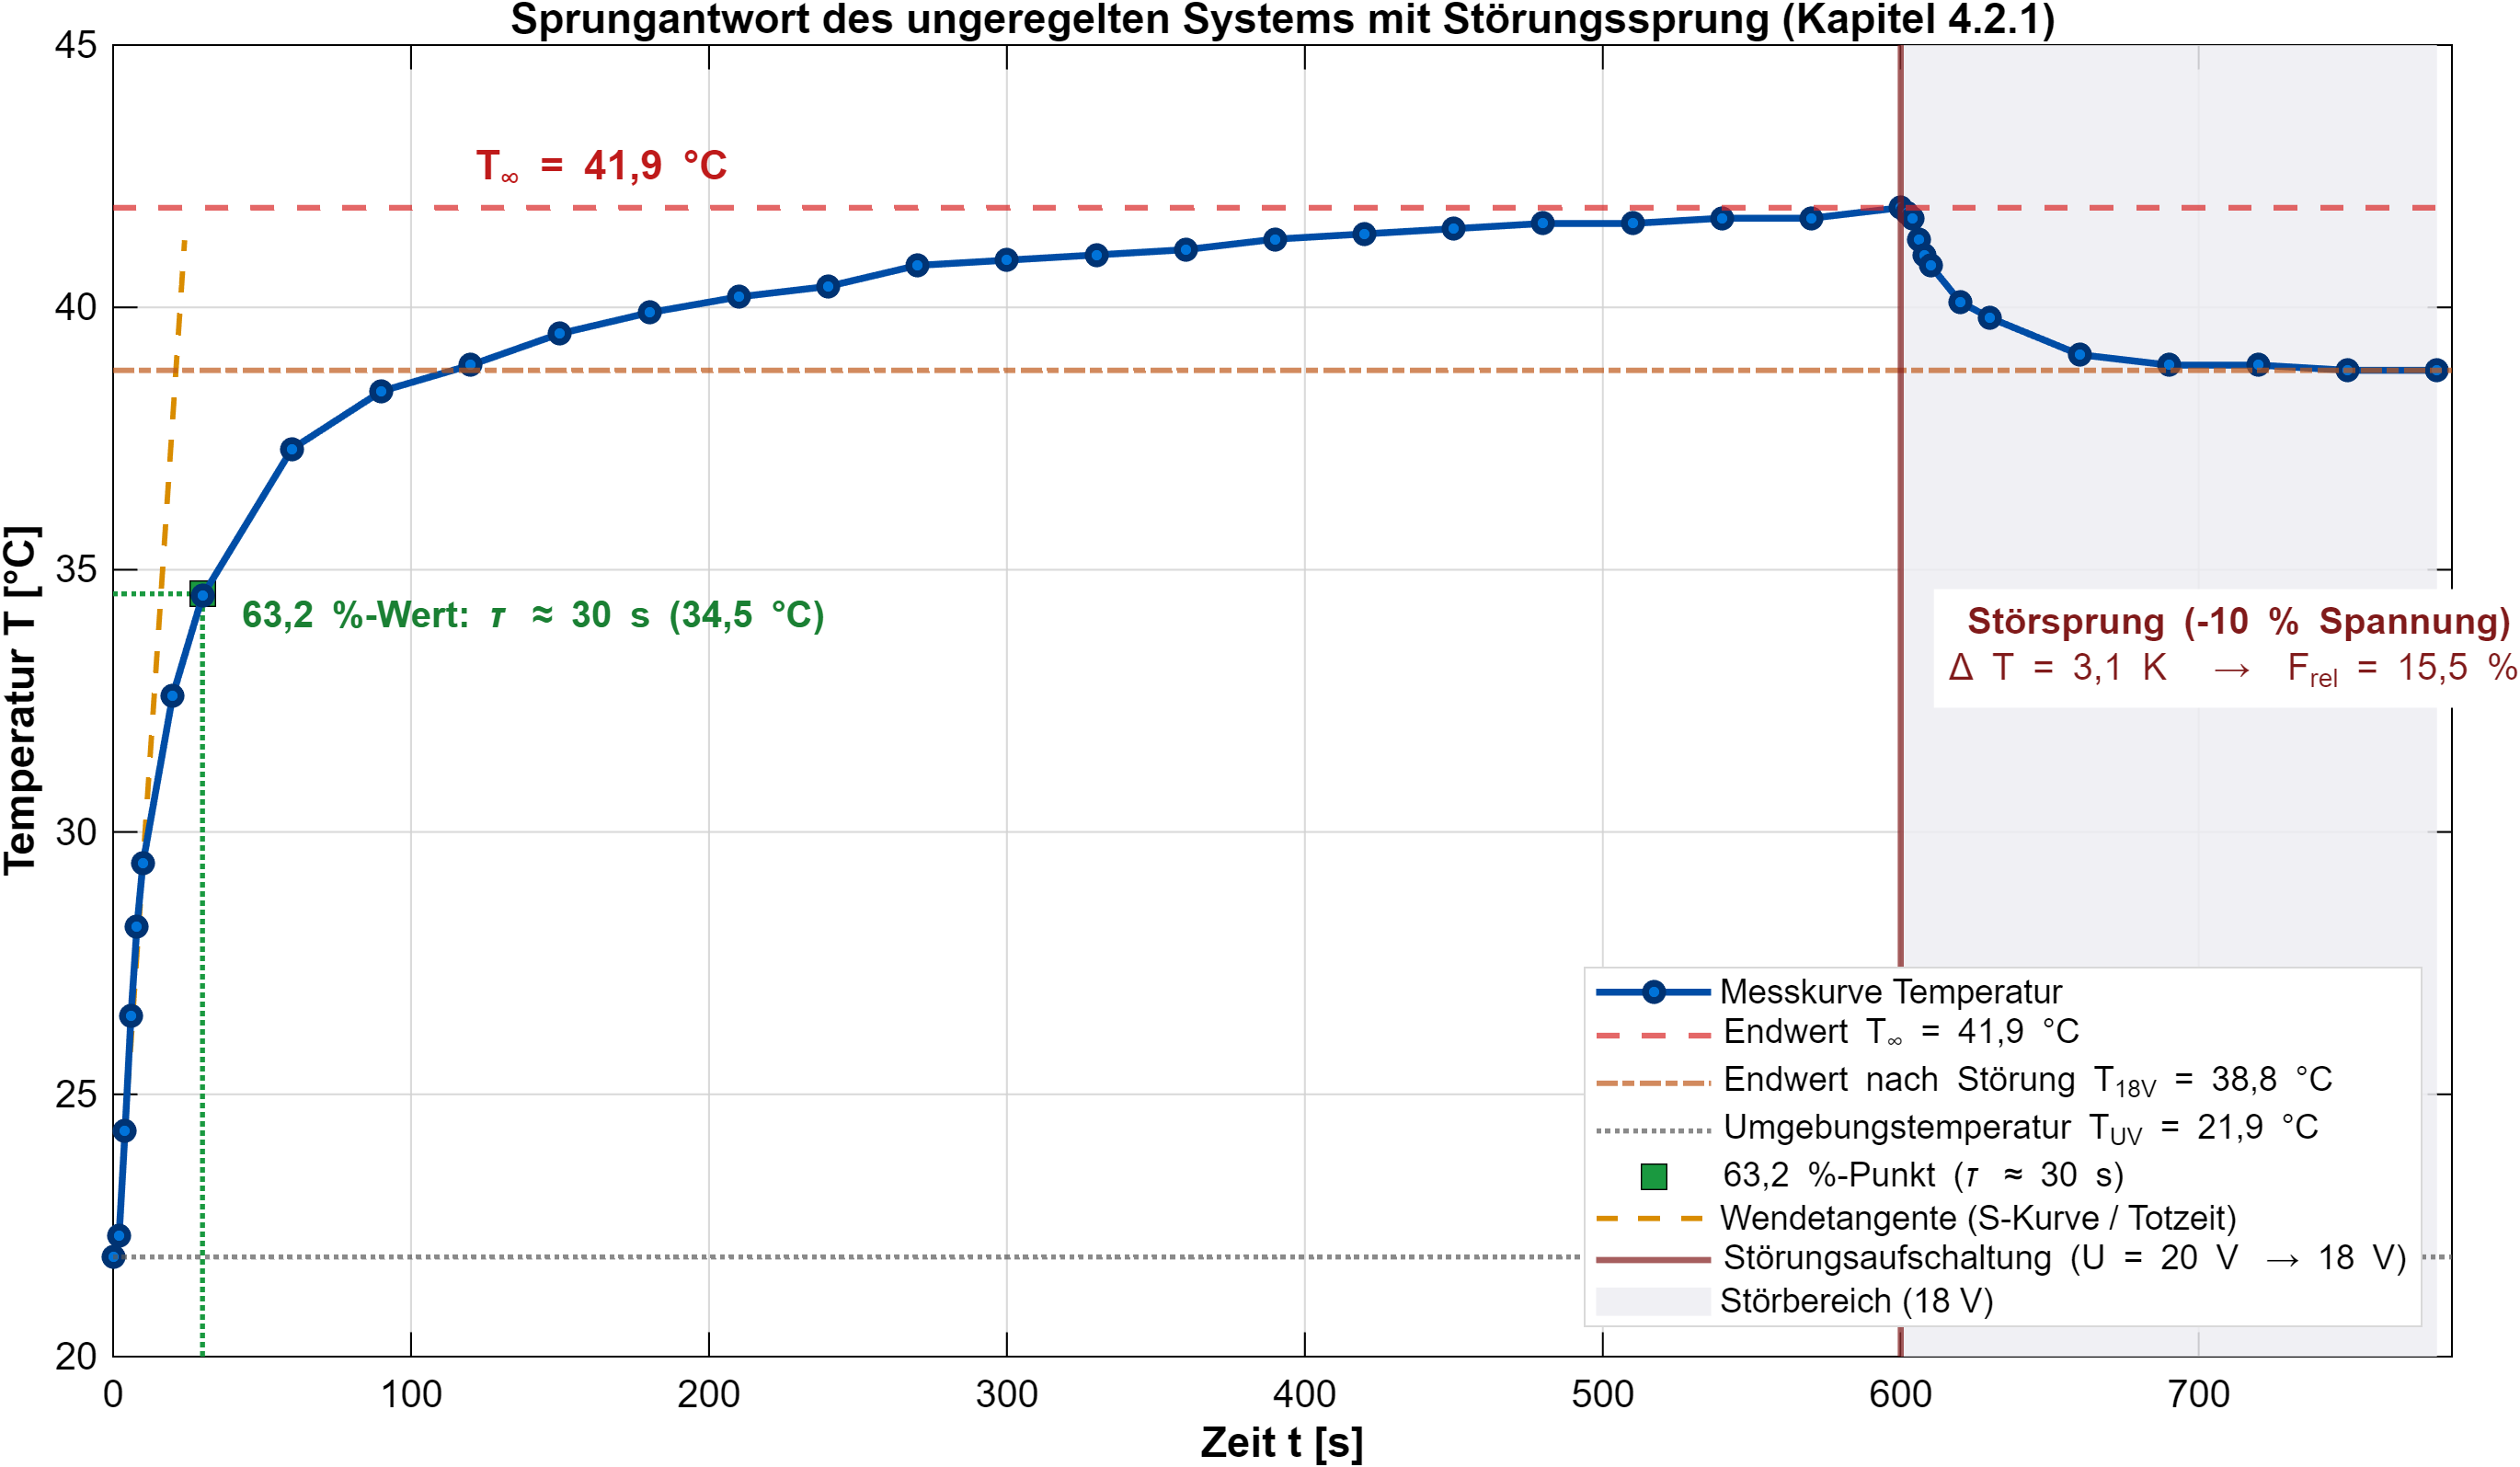
\includegraphics[width=0.96\textwidth,height=6.2cm,keepaspectratio]{sprungantwort_auswertung.png}
\caption{Gemessene Sprungantwort ($20\,\text{V}$) mit Störsprung ($18\,\text{V}$ ab $600\,\text{s}$), $63{,}2\,\%$-Kennwert und Wendetangente.}
\label{fig:sprungantwort}
\end{figure}

\clearpage

% ##############################################################################
% SEITE 2: MESSDATEN UNGEREGELT & MANUELLER BETRIEB
% ##############################################################################
\subsection{Messdaten des ungeregelten Betriebs}
Tabelle~\ref{tab:messdaten_sprung} dokumentiert den gemessenen Zeitverlauf des Aufheiz- und Störvorgangs.

\begin{table}[H]
\centering
\scriptsize
\caption{Messreihe der Sprungantwort bei $U = 20\,\text{V}$ sowie Störung bei $U = 18\,\text{V}$.}
\label{tab:messdaten_sprung}
\begin{tabular*}{\textwidth}{@{\extracolsep{\fill}}r *{13}{c}@{}}
\toprule
\textbf{Zeit [s]} & 0 & 2 & 4 & 6 & 8 & 10 & 20 & 30 & 60 & 90 & 120 & 150 & 180 \\
\textbf{T [$^\circ$C]} & 21,9 & 22,3 & 24,3 & 26,5 & 28,2 & 29,4 & 32,6 & 34,5 & 37,3 & 38,4 & 38,9 & 39,5 & 39,9 \\
\midrule
\textbf{Zeit [s]} & 210 & 240 & 270 & 300 & 330 & 360 & 390 & 420 & 450 & 480 & 510 & 540 & \textbf{600} \\
\textbf{T [$^\circ$C]} & 40,2 & 40,4 & 40,8 & 40,9 & 41,0 & 41,1 & 41,3 & 41,4 & 41,5 & 41,6 & 41,6 & 41,7 & \textbf{41,9} \\
\midrule
\multicolumn{14}{c}{\textbf{Störungsaufschaltung: Reduktion der Heizspannung auf $18\,\text{V}$ (ab $t = 600\,\text{s}$)}} \\
\textbf{Zeit $\Delta t$ [s]} & 0 & 2 & 4 & 6 & 8 & 10 & 20 & 30 & 60 & 90 & 120 & 150 & \textbf{180} \\
\textbf{T [$^\circ$C]} & 41,9 & 41,8 & 41,7 & 41,3 & 41,0 & 40,8 & 40,1 & 39,8 & 39,1 & 38,9 & 38,9 & 38,8 & \textbf{38,8} \\
\bottomrule
\end{tabular*}
\end{table}

\subsection{Ermittlung der Zeitkonstanten und Streckenmodellierung}
Für ein $\text{PT}_1$-System mit der Sprungantwort $T(t) = T_{\text{UV}} + \Delta T_{\infty} (1 - \mathrm{e}^{-t/\tau})$ wurden zwei Auswerteverfahren angewandt:
\begin{enumerate}
    \item \textbf{Verfahren 1 ($63{,}2\,\%$-Methode):} Der Sprung beträgt $\Delta T_{\infty} = T_{20\text{V}} - T_{\text{UV}} = 41{,}9\,^\circ\text{C} - 21{,}9\,^\circ\text{C} = 20{,}0\,\text{K}$.
    \begin{equation}
        T(\tau) = T_{\text{UV}} + 0{,}632 \cdot \Delta T_{\infty} = 21{,}9\,^\circ\text{C} + 12{,}64\,\text{K} = 34{,}54\,^\circ\text{C} \quad \implies \quad \mathbf{\tau \approx 30\,\text{s}}
    \end{equation}
    Der $90\,\%$-Wert $\Delta T_{90\,\%} = 18{,}0\,\text{K}$ ($T = 39{,}9\,^\circ\text{C}$) wird bei $\mathbf{t_{90\,\%} = 180\,\text{s}}$ erreicht.
    \item \textbf{Verfahren 2 (Wendetangentenverfahren):} Anlegen einer Tangente an die maximale Steigung ergibt eine Verzugszeit von $T_u \approx 1{,}2\,\text{s}$ und eine Ausgleichszeit von $T_g \approx 25\,\text{s}$.
\end{enumerate}
\textbf{Physikalische Begründung der Abweichung:} Das reale Rohr stellt \textbf{kein ideales $\text{PT}_1$-Glied} dar, sondern ein $\mathbf{\text{PT}_n}$-Glied höherer Ordnung mit Totzeit $T_t$:
\begin{equation}
    G_S(s) = \frac{K_S \cdot \mathrm{e}^{-s T_t}}{(1 + s T_{\text{Heizwendel}})(1 + s T_{\text{Rohrwand}})(1 + s T_{\text{Sensor}})}
\end{equation}
Die Wärmekapazitäten der Rohrwandung sowie die Strömungslaufzeit der Heißluft im Schlauch rufen die typische S-Kurve mit Anfangsverzug hervor. Zudem stellt sich das endgültige thermische Gleichgewicht erst nach über $30\,\text{min}$ ein, weshalb die 10-Minuten-Messung ein Quasigleichgewicht darstellt.

\subsection{Berechnung des relativen Fehlers bei Störungsaufschaltung}
Durch das Absenken der Heizspannung um $10\,\%$ fällt die Endtemperatur um $F_{\text{abs}} = 41{,}9\,^\circ\text{C} - 38{,}8\,^\circ\text{C} = 3{,}1\,\text{K}$.
\begin{tcolorbox}[title=\textbf{Vorbereitungsfrage: Sinnvolle Definition des relativen Temperaturfehlers}]
Da die Celsius-Skala einen willkürlich gewählten physikalischen Nullpunkt besitzt ($0\,^\circ\text{C}$), würde ein Bezug auf die Gradzahl in Celsius physikalisch wertlose Resultate liefern. Der relative Fehler muss physikalisch zwingend auf die \textbf{tatsächlich erzeugte Temperaturüberhöhung gegenüber der Raumtemperatur} bezogen werden:
\begin{equation}
    F_{\text{rel}} = \frac{F_{\text{abs}}}{T_{\text{End}} - T_{\text{UV}}} = \frac{T_{20\text{V}} - T_{18\text{V}}}{T_{20\text{V}} - T_{\text{UV}}} = \frac{3{,}1\,\text{K}}{41{,}9\,^\circ\text{C} - 21{,}9\,^\circ\text{C}} = \frac{3{,}1\,\text{K}}{20{,}0\,\text{K}} = \mathbf{15{,}5\,\%}
\end{equation}
\end{tcolorbox}
Wegen der quadratischen Abhängigkeit der Heizleistung $P = U^2 / R$ bewirkt eine $10\,\%$-Spannungsreduktion einen Leistungsabfall um ca. $19\,\%$, was beim ungeregelten System direkt zu einem hohen relativen Temperaturfehler von $15{,}5\,\%$ führt.

\section{Manueller Betrieb (Mensch als Regler)}
Im manuellen Betrieb sollte der Bediener über das Stellrad am Netzteil $T = 45{,}0\,^\circ\text{C}$ einstellen und für mindestens 2 Minuten innerhalb von $\pm 0{,}2\,^\circ\text{C}$ stabil halten.
\begin{itemize}
    \item \textbf{Benötigte Einregelzeit bis zum dauerhaften Halten:} $\mathbf{t_{\text{manuell}} = 65\,\text{s}}$ (über eine Minute).
    \item \textbf{Erkenntnis:} Infolge der thermischen Trägheit und Totzeit reagiert der Sensor verzögert. Der Mensch neigt zu starkem Übersteuern ($>46\,^\circ\text{C}$) mit nachfolgenden oszillierenden Gegenkorrekturen.
\end{itemize}

\clearpage

% ##############################################################################
% SEITE 3: ZIEGLER-NICHOLS & GEREGELTER BETRIEB
% ##############################################################################
\section{Reglerparametrierung nach Ziegler/Nichols (Schwingungsversuch)}
Bei $U = 25\,\text{V}$ und Sollwert $W = 45\,^\circ\text{C}$ wurde das System im geschlossenen Regelkreis als reiner P-Regler betrieben. Die Verstärkung $K_P$ wurde gesteigert, um die Stabilitätsgrenze experimentell zu ermitteln:

\begin{table}[H]
\centering
\small
\caption{Ermittlung der kritischen Verstärkung $K_{P,\text{krit}}$ am P-Regler ($W = 45\,^\circ\text{C}$).}
\label{tab:zn_schwingung}
\begin{tabular*}{\textwidth}{@{\extracolsep{\fill}}l *{8}{c} r@{}}
\toprule
\textbf{Einstellung $K_P$} & 1 & 2 & 4 & 8 & 16 & 32 & 64 & 50 & \textbf{40} \\
\midrule
\textbf{Temperatur [$^\circ$C]} & 28,3 & 31,0 & 34,5 & 38,1 & 41,1 & 43,0 & ROT & ROT & \textbf{Dauerschwingung} \\
\textbf{Periodendauer $T$} & -- & -- & -- & -- & -- & -- & -- & -- & $\mathbf{T_{\text{krit}} = 8{,}3\,\text{s}}$ \\
\bottomrule
\end{tabular*}
\end{table}

Bei $K_P = 40$ traten kontinuierliche, ungedämpfte Schwingungen auf:
\begin{equation}
    K_{P,\text{krit}} = 40 \qquad \text{und} \qquad T_{\text{krit}} = 8{,}3\,\text{s}
\end{equation}
Gemäß den Einstellregeln von Ziegler und Nichols errechnen sich die Reglerparameter:

\begin{table}[H]
\centering
\small
\caption{Berechnete Parameter für P-, PI- und PID-Regler nach Ziegler/Nichols.}
\label{tab:zn_parameter}
\begin{tabularx}{\textwidth}{l X X X c c c}
\toprule
\textbf{Reglertyp} & \textbf{Formel $K_P$} & \textbf{Formel $T_N$} & \textbf{Formel $T_V$} & \textbf{Wert $K_P$} & \textbf{Wert $T_N$} & \textbf{Wert $T_V$} \\
\midrule
\textbf{P-Regler}   & $0{,}5 \cdot K_{P,\text{krit}}$  & --                         & --                          & \textbf{20} & -- & -- \\
\textbf{PI-Regler}  & $0{,}45 \cdot K_{P,\text{krit}}$ & $0{,}85 \cdot T_{\text{krit}}$ & --                      & \textbf{18} & \textbf{7,1 s} & -- \\
\textbf{PID-Regler} & $0{,}6 \cdot K_{P,\text{krit}}$  & $0{,}5 \cdot T_{\text{krit}}$  & $0{,}12 \cdot T_{\text{krit}}$ & \textbf{24} & \textbf{4,2 s} & \textbf{1,0 s} \\
\bottomrule
\end{tabularx}
\end{table}

\section{Geregelter Betrieb im experimentellen Vergleich}
Das Führungsverhalten wurde anhand eines Sollwertsprungs von $W_L = 35\,^\circ\text{C}$ auf $W_H = 45\,^\circ\text{C}$ ($25\,\text{V}$) untersucht. Nach dem Einschwingen wurde die Heizspannung um $10\,\%$ auf $22{,}5\,\text{V}$ reduziert (Störsprung).

\begin{table}[H]
\centering
\small
\caption{Messwerte des Führungs- und Störverhaltens im geregelten Betrieb.}
\label{tab:reglervergleich}
\begin{tabular*}{\textwidth}{@{\extracolsep{\fill}}lcccccc@{}}
\toprule
\textbf{Reglertyp} & \textbf{Endtemp. $T_{H25}$} & \textbf{Einschwingzeit $t_{\text{ein}}$} & \textbf{Überschwingen} & \textbf{Temp. $T_{H22{,}5}$} & \textbf{Störfehler $F_{\text{abs}}$} & \textbf{Störfehler $F_{\text{rel}}$} \\
\midrule
\textbf{P-Regler}   & $42{,}3\,^\circ\text{C}$ & $25\,\text{s}$ & keines & $41{,}5\,^\circ\text{C}$ & $0{,}8\,\text{K}$ & \textbf{3,9\,\%} \\
\textbf{PI-Regler}  & $45{,}0\,^\circ\text{C}$ & $\mathbf{20\,\text{s}}$ & keines & $45{,}0\,^\circ\text{C}$ & $0{,}0\,\text{K}$ & \textbf{0,0\,\%} \\
\textbf{PID-Regler} & $45{,}0\,^\circ\text{C}$ & $22\,\text{s}$ & vorhanden & $45{,}0\,^\circ\text{C}$ & $0{,}0\,\text{K}$ & \textbf{0,0\,\%} \\
\bottomrule
\end{tabular*}
\end{table}

\begin{figure}[H]
\centering
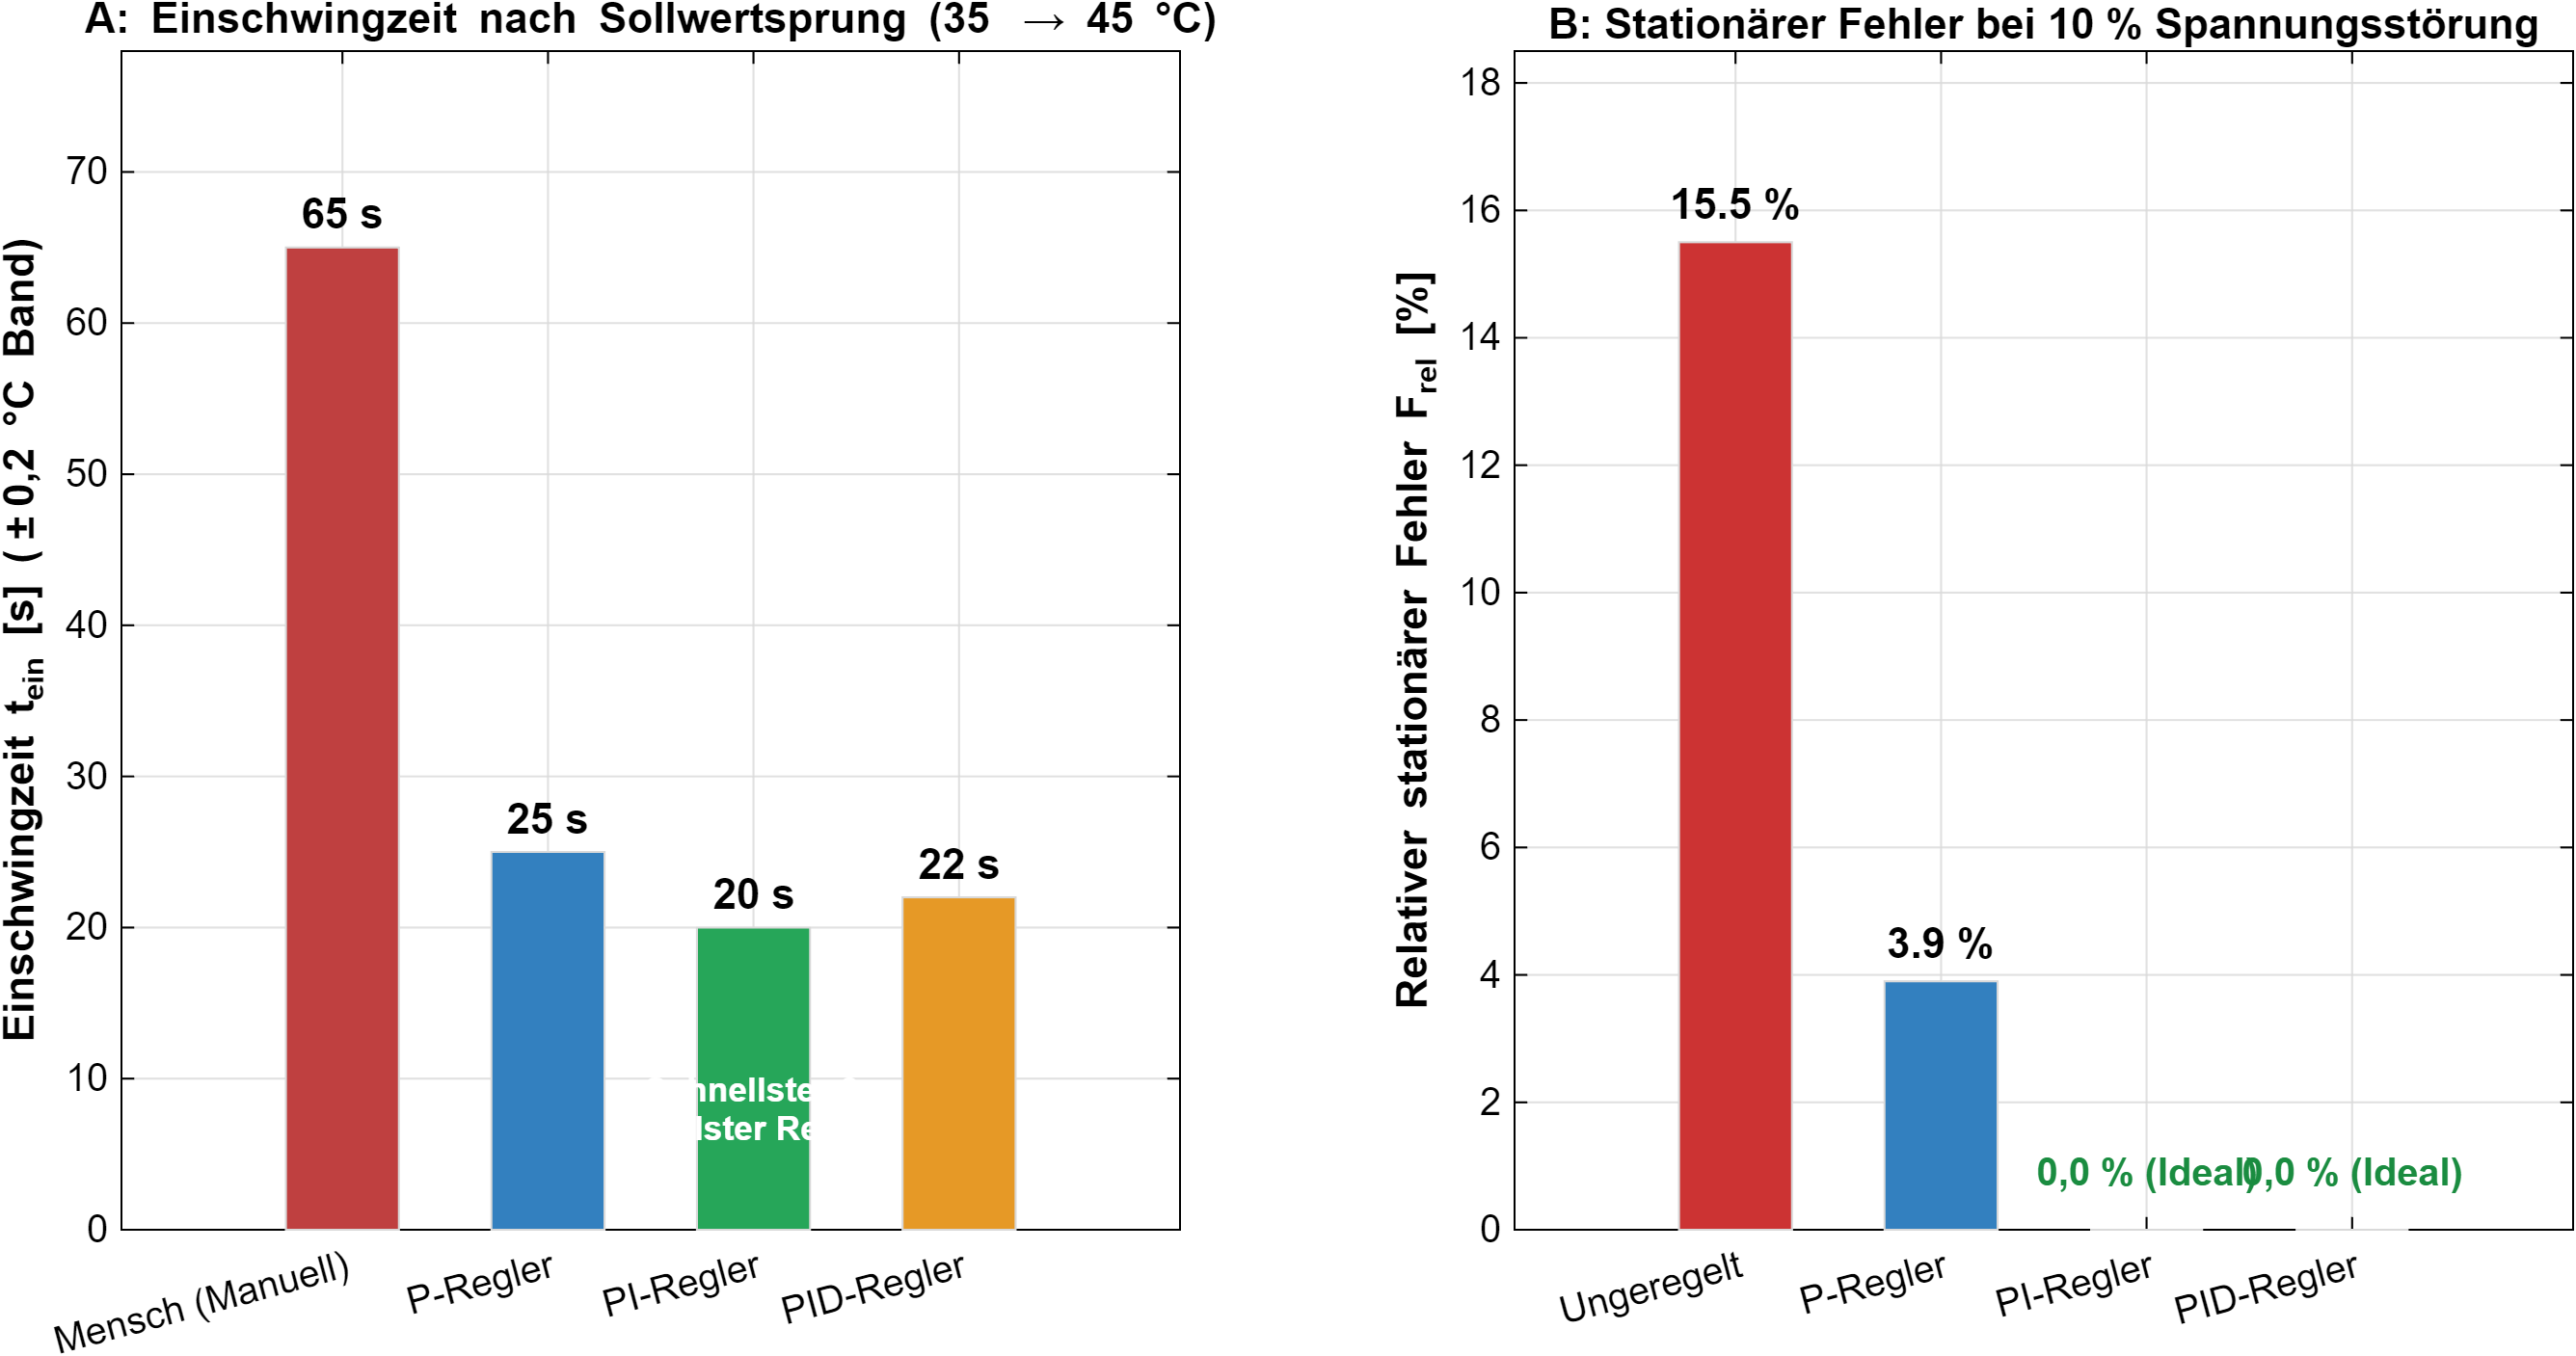
\includegraphics[width=0.96\textwidth,height=5.4cm,keepaspectratio]{reglervergleich.png}
\caption{Vergleichsanalyse der Einschwingzeiten (Diagramm A) und der stationären Störabweichung (Diagramm B).}
\label{fig:reglervergleich}
\end{figure}

\clearpage

% ##############################################################################
% SEITE 4: DISKUSSION & SYSTEMVERGLEICH
% ##############################################################################
\subsection{Vergleichende Analyse der Reglerstrukturen}
\begin{itemize}
    \item \textbf{P-Regler:}
    Zeigt ein gutmütiges, aperiodisches Einschwingen ($t_{\text{ein}} = 25\,\text{s}$), besitzt jedoch eine prinzipbedingte \textbf{bleibende Regelabweichung}:
    \begin{equation}
        e_{\infty} = W_H - T_{H25} = 45{,}0\,^\circ\text{C} - 42{,}3\,^\circ\text{C} = \mathbf{2{,}7\,\text{K}}
    \end{equation}
    Unter Störung fällt die Temperatur weiter auf $41{,}5\,^\circ\text{C}$ ab ($F_{\text{rel}} = 3{,}9\,\%$). Ein reiner P-Regler benötigt zwingend eine bleibende Abweichung $e \neq 0$, um an seinem Ausgang eine Stellgröße $Y = K_P \cdot e > 0$ zu halten. Eine Erhöhung von $K_P$ verringert zwar den Fehler, rückt das System aber gefährlich nah an die Stabilitätsgrenze ($K_{P,\text{krit}} = 40$).
    \item \textbf{PI-Regler:}
    Der I-Anteil integriert die verbleibende Regelabweichung auf, bis diese exakt verschwindet ($e_{\infty} = 0$). Sowohl die Führungsgröße ($45{,}0\,^\circ\text{C}$) als auch die $10\,\%$-Spannungsstörung werden \textbf{vollständig fehlerfrei ($0{,}0\,\text{K}$ Abweichung, $0{,}0\,\%$ Störfehler)} ausgeregelt. Mit einer Einschwingzeit von $\mathbf{t_{\text{ein}} = 20\,\text{s}}$ ist der PI-Regler der dynamisch schnellste und robusteste Regler.
    \item \textbf{PID-Regler:}
    Erzielt ebenfalls stationäre Genauigkeit ($e_{\infty} = 0$). Allerdings tritt beim Sollwertsprung ein merkliches Überschwingen auf, weshalb das finale Einregeln in das schmale Toleranzband von $\pm 0{,}2\,^\circ\text{C}$ mit $\mathbf{t_{\text{ein}} = 22\,\text{s}}$ etwas länger dauert als beim PI-Regler.
\end{itemize}

\subsection{Kritische Reflexion: Warum ist der PI-Regler hier schneller als der PID-Regler?}
In der linearen Regelungstheorie gilt die Daumenregel, dass ein D-Anteil über Phasenvorhalt schnelleres Einschwingen ermöglicht. Die im Versuch dokumentierte Umkehrung ($t_{\text{ein, PI}} = 20\,\text{s} < t_{\text{ein, PID}} = 22\,\text{s}$) basiert auf zwei systemischen Faktoren:
\begin{enumerate}
    \item \textbf{Aggressivität der Ziegler-Nichols-Parametrierung:} Ziegler-Nichols strebt klassisch ein Einschwingverhalten mit ca. $20\,\%$ Überschwingen an. Beim PID-Regler führt die Kombination aus höherem $K_P = 24$ (vs. $K_{P,\text{PI}} = 18$) und dem differenzierenden Anteil zu einem massiven anfänglichen Stellgrößenstoß, der die Temperatur über das Ziel schießen lässt.
    \item \textbf{Kriterium des schmalen Toleranzbands ($\pm 0{,}2\,^\circ\text{C}$):} Der PI-Regler nähert sich aperiodisch von unten an und verbleibt sofort dauerhaft im Band. Der PID-Regler erreicht die $45\,^\circ\text{C}$ zwar früher, verlässt den engen Korridor aber durch das Überschwingen wieder und benötigt Nachschwingzeit zum Wiedereintritt.
\end{enumerate}

\subsection{Gegenüberstellung: Steuerung vs. Mensch vs. Regelalgorithmus}
Tabelle~\ref{tab:systemvergleich} stellt die Gesamtergebnisse des Experiments gegenüber.

\begin{table}[H]
\centering
\footnotesize
\caption{Systemvergleich zwischen ungeregeltem, manuellem und geregeltem Betrieb.}
\label{tab:systemvergleich}
\begin{tabularx}{\textwidth}{p{3.0cm} *{4}{>{\raggedright\arraybackslash}X}}
\toprule
\textbf{Kriterium} & \textbf{Ungeregelt (Steuerung)} & \textbf{Mensch (Manuell)} & \textbf{P-Regler} & \textbf{PI-Regler (Optimum)} \\
\midrule
\textbf{Führungsfehler} & Groß (Arbeitspunkt) & $\pm 0{,}2\,\text{K}$ (nach Einregeln) & $2{,}7\,\text{K}$ bleibend & \textbf{0,0 K (Exakt)} \\
\textbf{Einschwingzeit} & $>180\,\text{s}$ ($90\,\%$) & $65\,\text{s}$ & $25\,\text{s}$ & \textbf{20 s} \\
\textbf{Störfehler ($-10\,\%$)} & $F_{\text{rel}} = 15{,}5\,\%$ & Manuelles Nachstellen & $F_{\text{rel}} = 3{,}9\,\%$ & \textbf{0,0 \% (Vollständig)} \\
\textbf{Stabilität / Dynamik} & Aperiodisch träge & Hohe Oszillationen & Aperiodisch stabil & \textbf{Aperiodisch optimal} \\
\bottomrule
\end{tabularx}
\end{table}

\clearpage

% ##############################################################################
% SEITE 5: SYNTHESE UND WISSENSCHAFTLICHER ERKENNTNISGEWINN (TAKE-AWAYS)
% ##############################################################################
\section{Synthese und wissenschaftlicher Erkenntnisgewinn}
Dieser Abschnitt bündelt die zentralen wissenschaftlichen Erkenntnisse (Take-Aways) des Versuchs V1 und beantwortet die regelungstechnischen Testfragen.

\subsection{Systemtheoretische Pol-Nullstellen-Analyse (Wurzelortskurve)}
Die Ursache für die experimentellen Differenzen zwischen P, PI und PID lässt sich mathematisch in der komplexen $s$-Ebene erklären (Abbildung~\ref{fig:wok_analyse}):

\begin{figure}[H]
\centering
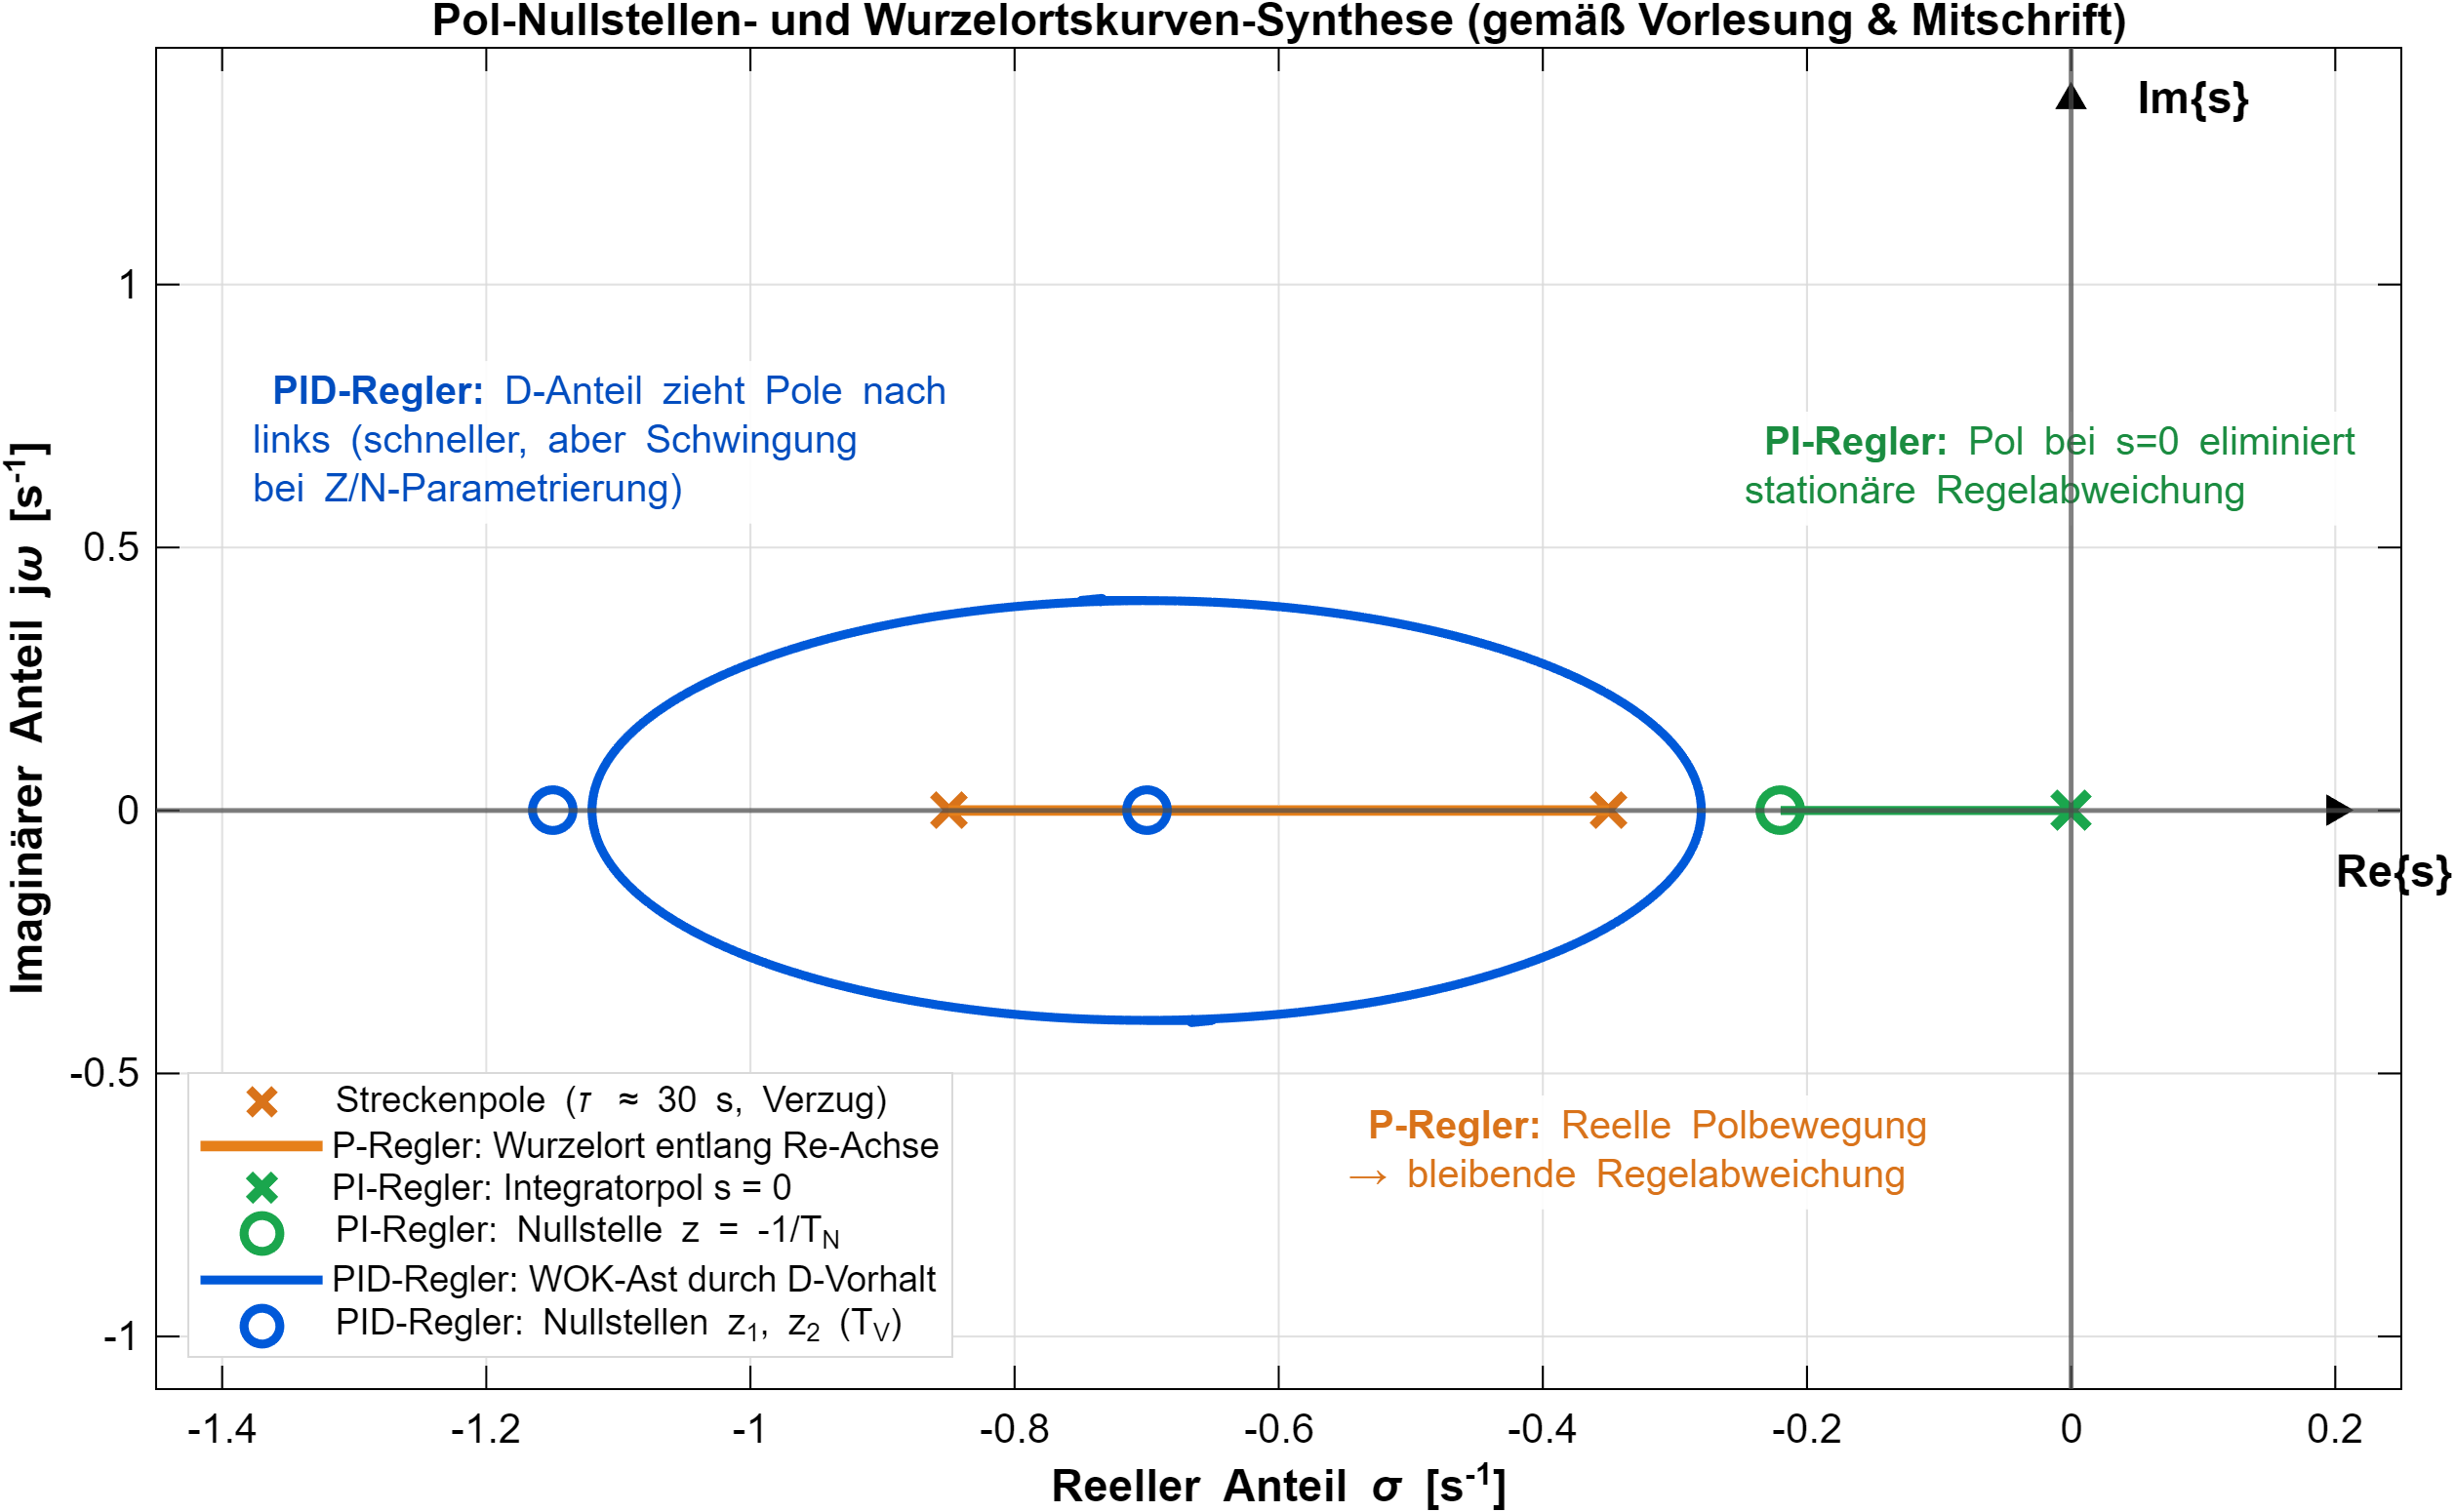
\includegraphics[width=0.92\textwidth,height=5.2cm,keepaspectratio]{wok_analyse.png}
\caption{Polstellen- und Wurzelortskurven-Synthese (WOK) für P-, PI- und PID-Regelung.}
\label{fig:wok_analyse}
\end{figure}

\begin{itemize}
    \item \textbf{P-Regler:} Die Wurzelortskurve verläuft auf der negativen reellen Achse. Höhere Verstärkung beschleunigt das System, kann aber wegen fehlenden Integrators die statische Abweichung nicht eliminieren.
    \item \textbf{PI-Regler:} Der Integratorpol im Ursprung ($s = 0$) sorgt für unendliche statische Kreisverstärkung und erzwingt $e_{\infty} = 0$. Die Nullstelle bei $s = -1/T_N$ zieht den Polast nach links; die dominanten Pole verbleiben reell, was das aperiodische Einschwingen ohne Überschwingen erklärt.
    \item \textbf{PID-Regler:} Der Vorhalt $T_V$ schaltet zwei Nullstellen auf. Die Wurzelortskurve biegt kreisförmig in die komplexe Halbebene aus. Dies erhöht die Bandbreite, erzeugt jedoch konjugiert-komplexe Pole $\sigma \pm \mathrm{j}\omega_d$, die bei Z/N für das Überschwingen verantwortlich sind.
\end{itemize}

\subsection{Beantwortung der Test- und Kolloquiumsfragen}
\begin{enumerate}
    \item \textbf{Grund für den Einsatz eines I-Anteils:} Ein I-Anteil besitzt bei Gleichgrößen ($\omega = 0$) unendliche Verstärkung ($G_I(0) \rightarrow \infty$). Dadurch treibt bereits die kleinste Abweichung $e(t)$ die Stellgröße unaufhörlich weiter, bis $e_{\infty} = 0$ exakt erreicht ist. Er eliminiert bleibende Fehler bei Führungs- und Störgrößensprüngen vollständig.
    \item \textbf{Grund für den Einsatz eines D-Anteils:} Der D-Anteil reagiert auf die Änderungsgeschwindigkeit $\frac{\mathrm{d}e}{\mathrm{d}t}$. Er wirkt prädiktiv (vorhaltend), bremst schnelle Temperaturdrifts frühzeitig ab und erzeugt Phasenreserve, um träge Strecken zu stabilisieren.
    \item \textbf{Vorgehen bei Ziegler-Nichols (Schwingungsmethode):}
    1.~Reinen P-Betrieb wählen ($T_N \rightarrow \infty, T_V = 0$). 2.~$K_P$ schrittweise erhöhen, bis Dauerschwingungen auftreten ($K_{P,\text{krit}}$). 3.~Periodendauer $T_{\text{krit}}$ messen. 4.~Parameter berechnen: $K_P = 0{,}45 \cdot K_{P,\text{krit}}$, $T_N = 0{,}85 \cdot T_{\text{krit}}$.
    \item \textbf{Vorteil der Pulsweitenmodulation (PWM) gegenüber linearer Stellgliedsteuerung:}
    Bei analoger Längsregelung fällt am Transistor eine Verlustleistung $P_V = (U_{\text{Netz}} - U_{\text{Last}}) \cdot I$ ab, die als extreme Abwärme verloren geht. Bei PWM arbeitet der FET als verlustarmer Schalter: voll gesperrt ($I = 0 \implies P_V = 0$) oder voll durchgeschaltet ($U_{DS} \approx 0 \implies P_V \approx 0$). Dies gewährleistet einen Wirkungsgrad von nahezu $100\,\%$.
\end{enumerate}

\subsection{Zusammenfassendes Fazit}
Der Versuch belegt eindrucksvoll die Überlegenheit eines geschlossenen Regelkreises gegenüber Steuerung und manuellem Eingriff. Während die manuelle Bedienung an Totzeit und thermischer Trägheit scheitert ($65\,\text{s}$ Einregelzeit), stabilisiert der industrielle Kompaktregler das System zuverlässig. Für die thermische Rohrstrecke erwies sich der \textbf{PI-Regler} mit $t_{\text{ein}} = 20\,\text{s}$ und $0\,\%$ stationärer Abweichung als die in jeder Hinsicht überlegene Reglerkonfiguration.

\end{document}
